7. \points{15} In this problem we will examine the bias-variance tradeoff through learning curves. Learning curves provide a valuable mechanism for evaluating the bias-variance tradeoff. Implement the \texttt{learningCurve()} function in \texttt{polyreg.py} to compute the learning curves for a given training/test set.  The \texttt{learningCurve(Xtrain, ytrain, Xtest, ytest, degree, regLambda)} function should take in the training data (\texttt{Xtrain}, \texttt{ytrain}), the testing data (\texttt{Xtest}, \texttt{ytest}), and values for the polynomial degree $d$ and regularization parameter $\lambda$. 

The function should return two arrays, \texttt{errorTrain} (the array of training errors) and \texttt{errorTest} (the array of testing errors).  The $i^{th}$ index (start from 0) of each array should return the training error (or testing error) for learning with $i +1$ training instances.  Note that the 0$^{th}$ index actually won't matter, since we typically start displaying the learning curves with two or more instances.


\vspace{.1in}
When computing the learning curves, you should learn on \texttt{Xtrain}[0:$i$] for $i = 1, \ldots, \text{numInstances}(\texttt{Xtrain})+1$, each time computing the testing error over the {\bf entire} test set.  There is no need to shuffle the training data, or to average the error over multiple trials -- just produce the learning curves for the given training/testing sets with the instances in their given order.  Recall that the error for regression problems is given by
\begin{equation}
\frac{1}{n} \sum_{i=1}^n (h_{\bm{\theta}}(\mathbf{x}_i) - y_i)^2 \enspace .
\end{equation}

Once the function is written to compute the learning curves, run the \texttt{test\_polyreg\_learningCurve.py} script to plot the learning curves for various values of $\lambda$ and $d$.  You should see plots similar to the following:
\begin{figure}[ht!]
      \centering
      \vspace{-1em}
      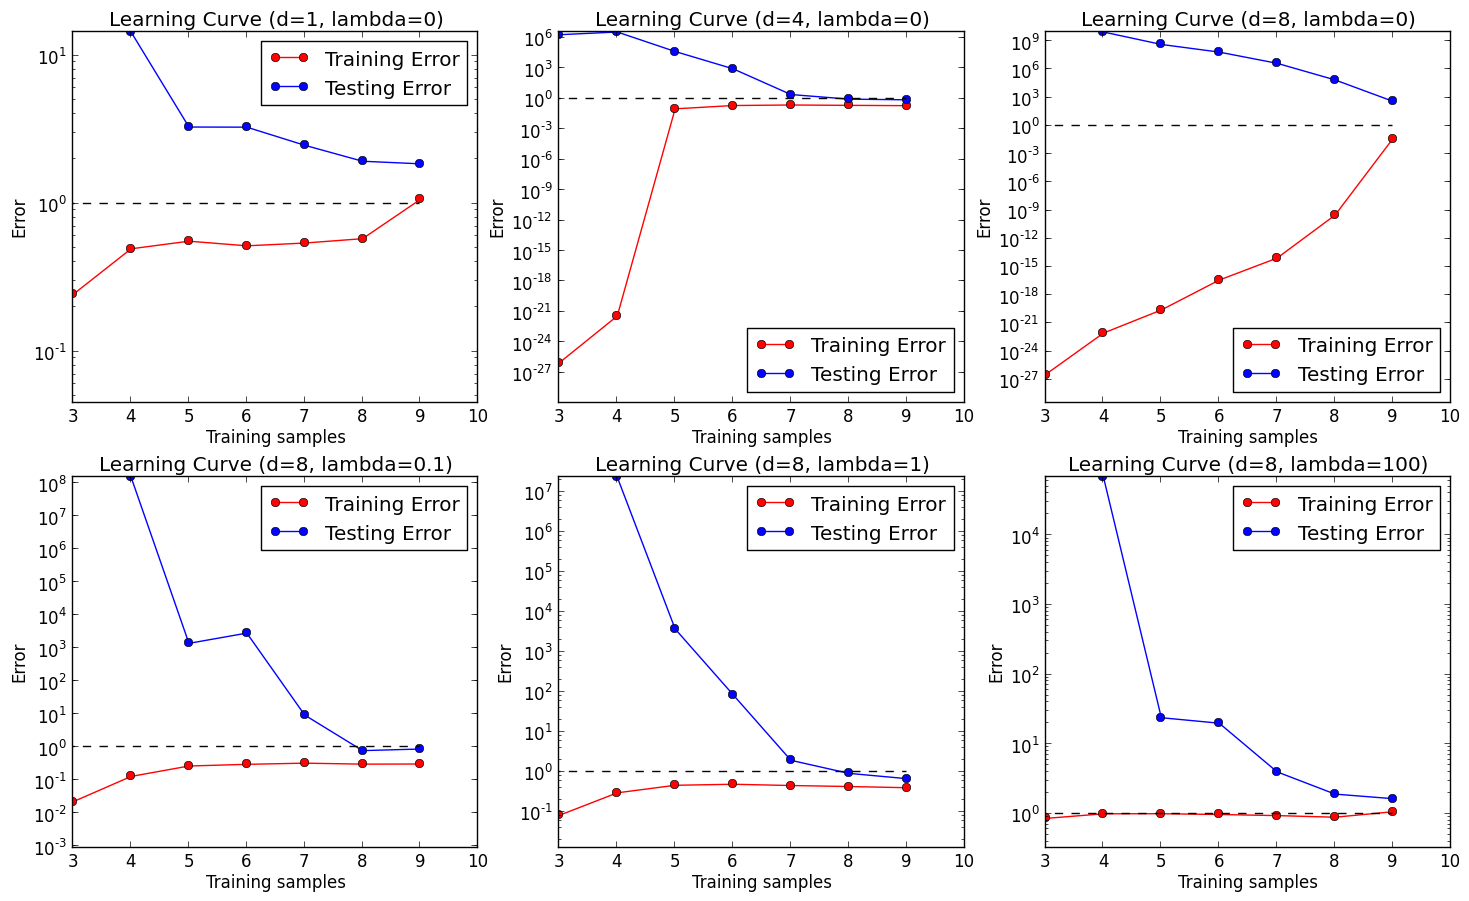
\includegraphics[width=\textwidth]{images/polyregLearningCurves.png}
      \vspace{-1em}
    \end{figure}

Notice the following:
\begin{itemize}
\item The y-axis is using a log-scale and the ranges of the y-scale are all different for the plots.  The dashed black line indicates the $y=1$ line as a point of reference between the plots.
\item The plot of the unregularized model with $d = 1$ shows poor training error, indicating a high bias (i.e., it is a standard univariate linear regression fit).
\item The plot of the unregularized model ($\lambda = 0$) with $d = 8$ shows that the training error is low, but that the testing error is high.  There is a huge gap between the training and testing errors caused by the model overfitting the training data, indicating a high variance problem.
\item As the regularization parameter increases (e.g., $\lambda = 1$) with $d = 8$, we see that the gap between the training and testing error narrows, with both the training and testing errors converging to a low value.  We can see that the model fits the data well and generalizes well, and therefore does not have either a high bias or a high variance problem.  Effectively, it has a good tradeoff between bias and variance.
\item Once the regularization parameter is too high ($\lambda = 100$), we see that the training and testing errors are once again high, indicating a poor fit.  Effectively, there is too much regularization, resulting in high bias.
\end{itemize}

\textbf{Please include both your code and the generated plots in your homework.} Make absolutely certain that you understand these observations, and how they relate to the learning curve plots.  In practice, we can choose the value for $\lambda$ via cross-validation to achieve the best bias-variance tradeoff.

\begin{quote}
    \FloatBarrier
    \begin{figure}
	\captionsetup{labelformat=empty}	
	\caption{Results of training and testing error over multiple degrees d and lambdas $\lambda$.}
	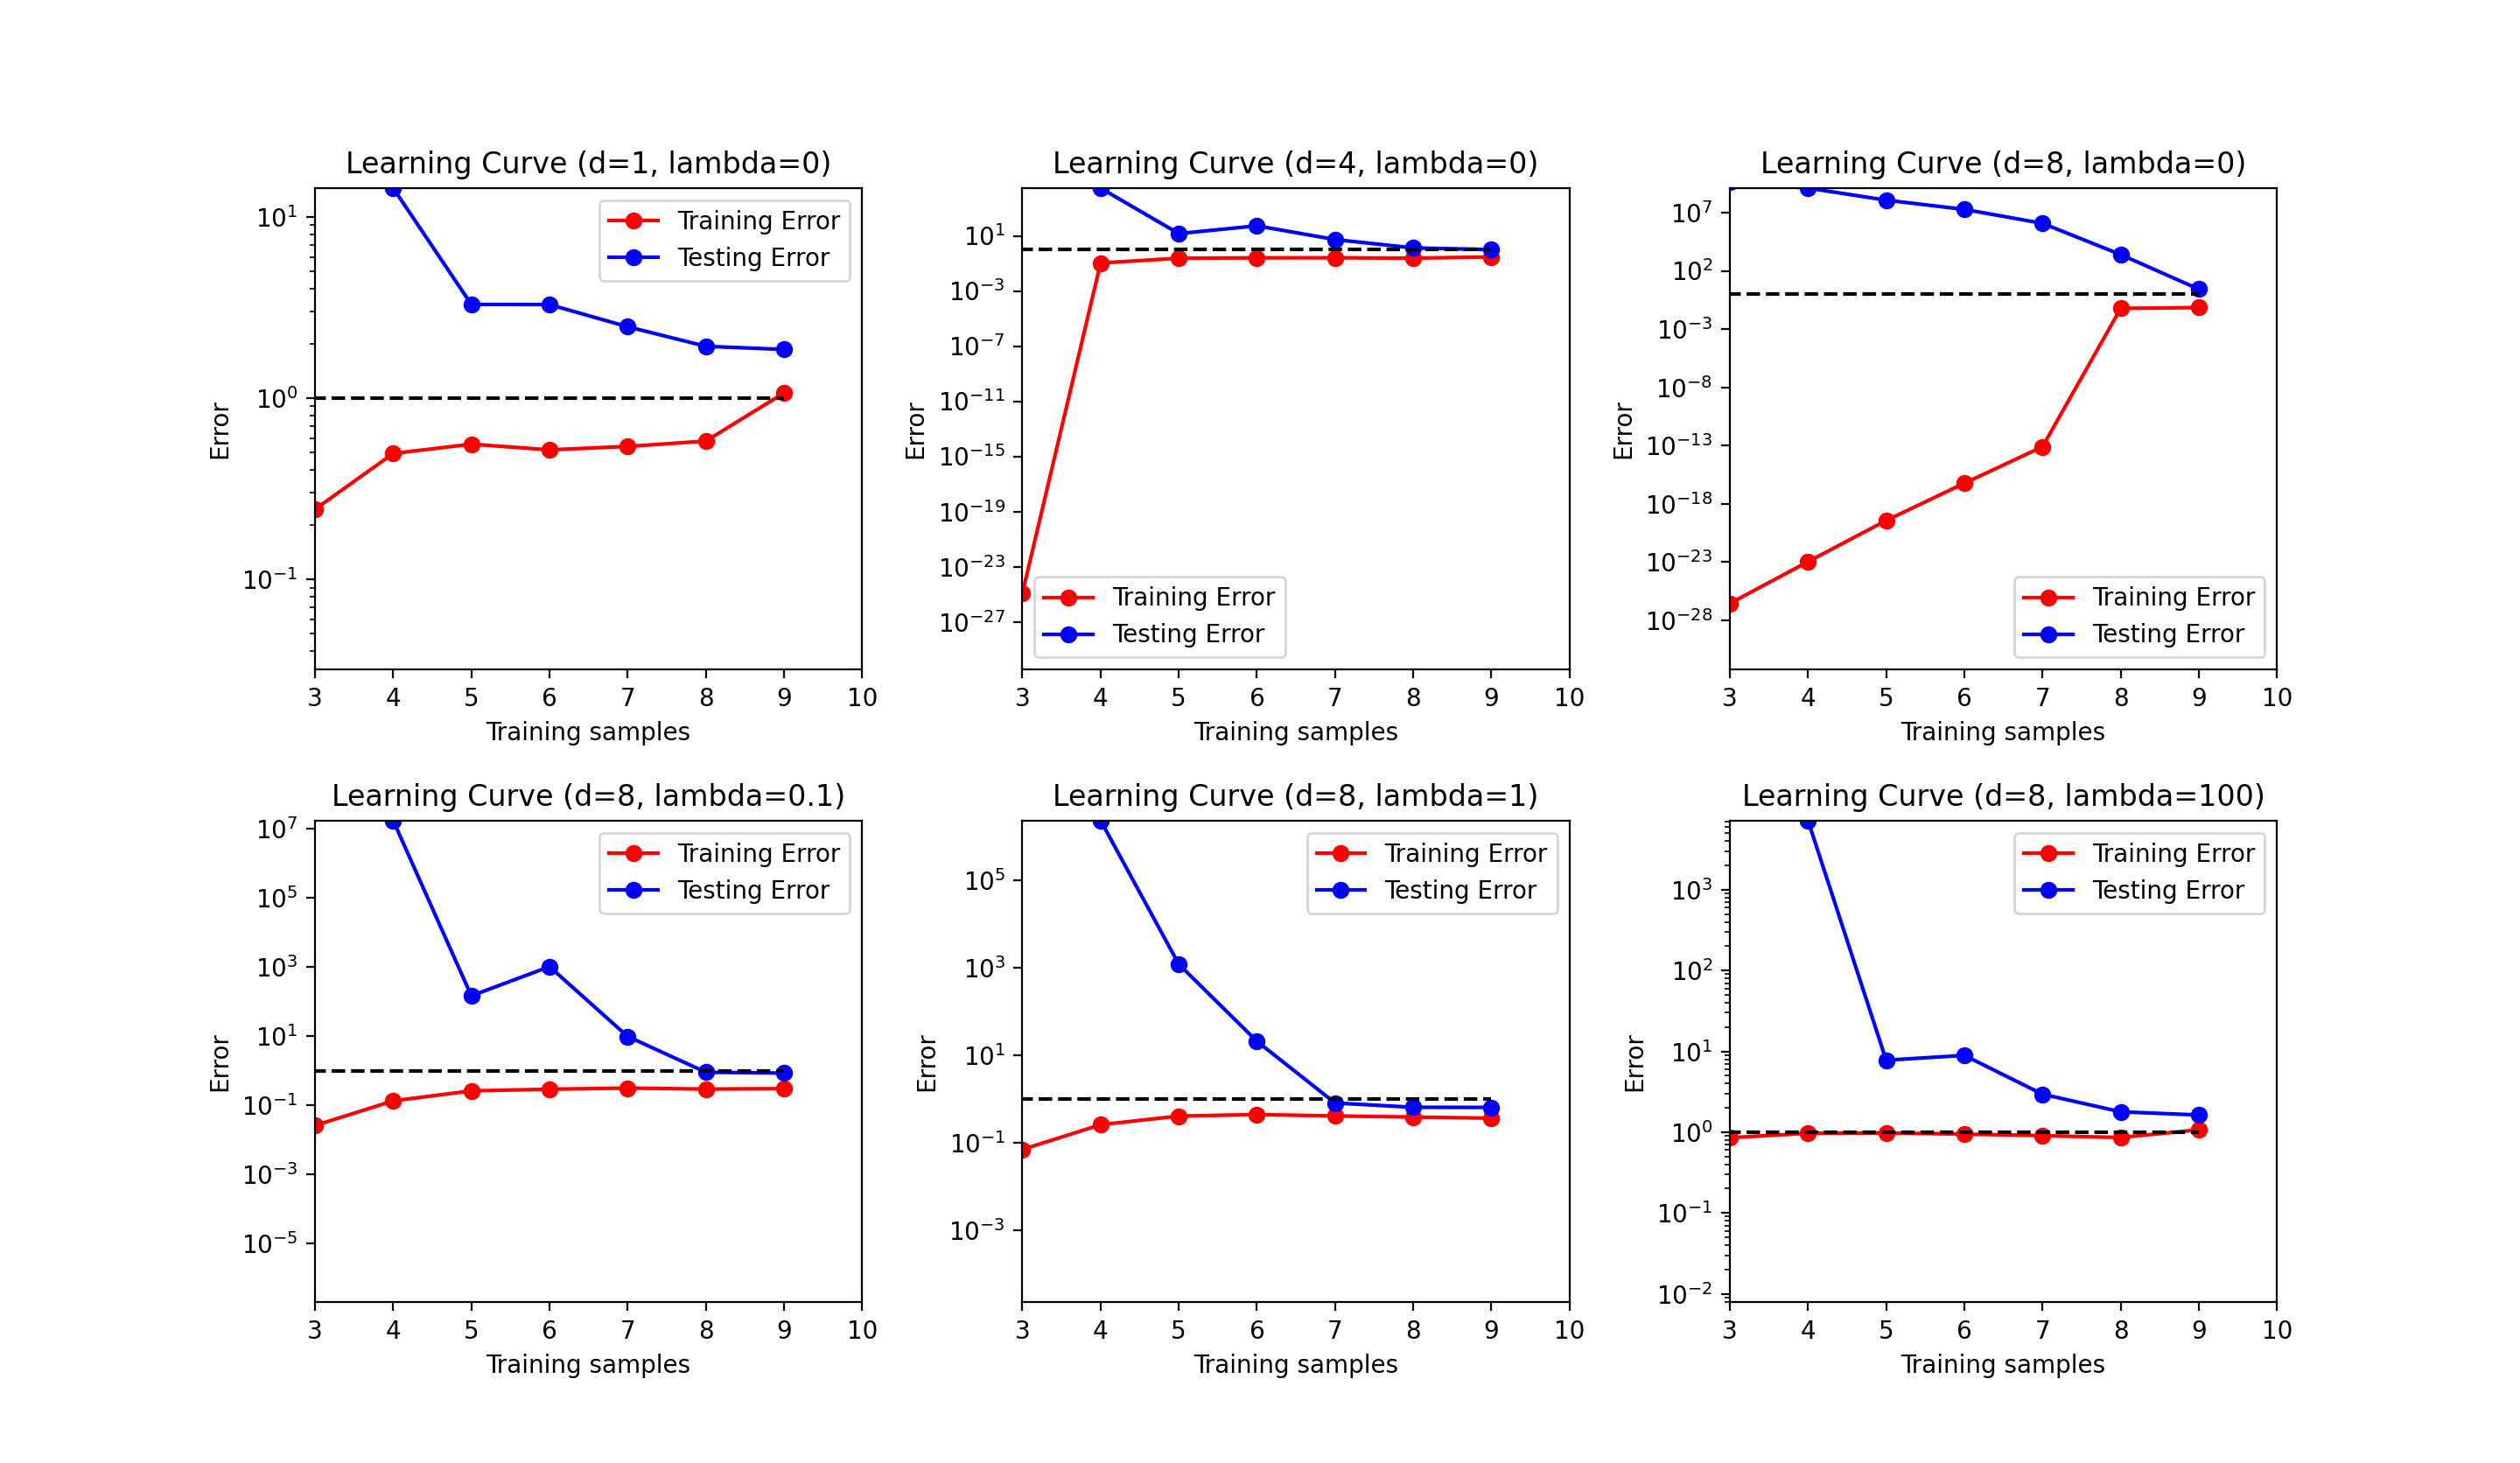
\includegraphics[scale=0.5]{./images/fig2.png} 
	\centering
    \end{figure}
    \FloatBarrier
    \begin{itemize}
	\item[] \lstinputlisting[language=Python]{body/polyreg.py}
    \end{itemize}
\end{quote}


